\section{Concrete Syntax}
\label{sec:slco:syntax}

\SLCO has both a textual and a graphical concrete syntax.
The graphical concrete syntax consists of communication diagrams, structure diagrams, and behavior diagrams.
The diagrams in Figures~\ref{fig:slco:SLCOExampleCommunication}, \ref{fig:slco:SLCOExampleStructure}, and~\ref{fig:slco:SLCOExampleSMS} show an example of an \SLCO model using the graphical syntax.
Below, we describe the model shown in these figures.

The communication diagram in Figure~\ref{fig:slco:SLCOExampleCommunication} shows two objects~\SLCOObject{p} and~\SLCOObject{q} that communicate over an asynchronous, lossless channel~\SLCOChannel{c1}, an asynchronous, lossy channel~\SLCOChannel{c2}, and a synchronous channel~\SLCOChannel{c3}.
Asynchronous, lossless channels, such as~\SLCOChannel{c1}, are denoted by dashed lines, asynchronous, lossy channels, such as~\SLCOChannel{c2}, are denoted by dotted lines, and synchronous channels, such as~\SLCOChannel{c3}, are denoted by solid lines.
The diagram shows that both objects have three ports.
The ports of object~\SLCOObject{p} are named~\SLCOPort{In1}, \SLCOPort{In2}, and~\SLCOPort{InOut}, and the ports of object~\SLCOObject{q} are named~\SLCOPort{Out1}, \SLCOPort{Out2}, and~\SLCOPort{InOut}.
Arrowheads indicate the directionality of channels: unidirectional channels have one arrowhead and bidirectional channels have two.
Object~\SLCOObject{q} can only send signals over channel~\SLCOChannel{c1} via its port~\SLCOPort{Out1}, for example, and object~\SLCOObject{p} can only receive signals sent over channel~\SLCOChannel{c1} via its port~\SLCOPort{In1}.
Channel~\SLCOChannel{c3}, however, can be used for communication in both directions.
Channel~\SLCOChannel{c1} can only be used to send and receive signals with a Boolean argument, channel~\SLCOChannel{c2} is restricted to signals with integer arguments, and channel~\SLCOChannel{c3} is restricted to signals with string arguments.
The figure also shows that object~\SLCOObject{p} is an instance of class~\SLCOClass{P} and that object~\SLCOObject{q} is an instance of class~\SLCOClass{Q}.

\begin{figure}[hbt]
 \centering
 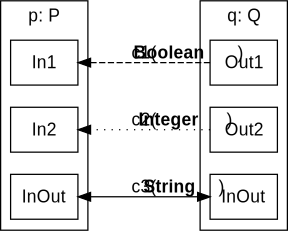
\includegraphics[scale=0.45]{slco/figs/CoreWithTime/Communication_CoreWithTime}
 \caption{Objects, ports, and channels of an \SLCO model}
 \label{fig:slco:SLCOExampleCommunication}
\end{figure}

The structure diagram in Figure~\ref{fig:slco:SLCOExampleStructure} shows the structure of classes~\SLCOClass{P} and~\SLCOClass{Q}.
Class~\SLCOClass{P} consists of three state machines (\SLCOStateMachine{Rec1}, \SLCOStateMachine{Rec2}, and \SLCOStateMachine{SendRec}), and class~\SLCOClass{Q} consists of one state machine (\SLCOStateMachine{Com}).
Furthermore, it shows that class~\SLCOClass{P} comprises an integer variable~\SLCOVariable{m} and that state machines~\SLCOClass{SendRec} and~\SLCOClass{Com} comprise a string variable~\SLCOVariable{s}.
The initial value of variable~\SLCOVariable{m} is $0$.
The initial values of the other variables are not specified, which means that they are initialized to empty strings as described above.

\begin{figure}[hbt]
  \centering
  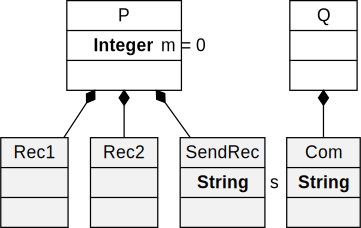
\includegraphics[scale=0.45]{slco/figs/CoreWithTime/Structure_CoreWithTime}
  \caption{Classes, state machines, and variables of an \SLCO model}
  \label{fig:slco:SLCOExampleStructure}
\end{figure}

\begin{figure}[hbt]
  \centering
  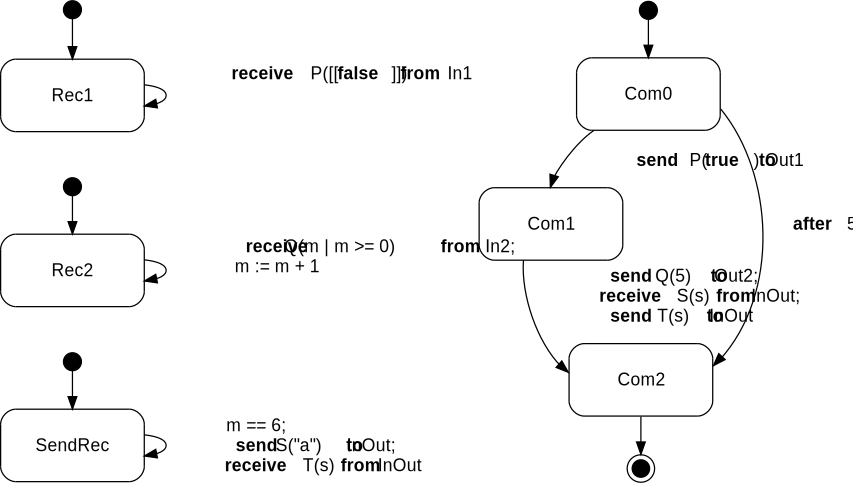
\includegraphics[scale=0.45]{slco/figs/CoreWithTime/Behavior_CoreWithTime}
  \caption{State machines of an \SLCO model}
  \label{fig:slco:SLCOExampleSMS}
\end{figure}

The behavior diagram in Figure~\ref{fig:slco:SLCOExampleSMS} shows the four state machines of our example model.
The three state machines on the left of this figure specify the behavior of object~\SLCOObject{p}, and the state machine on the right specifies the behavior of object~\SLCOObject{q}.
Initially, all of these state machines are in their initial states, which are named~\SLCOState{Rec1}, \SLCOState{Rec2}, \SLCOState{SendRec}, and~\SLCOState{Com0}.
The fact that these states are initial states is indicated by an incoming arrow from a solid black dot.
The black dot itself does not represent a separate state.

When state machine~\SLCOStateMachine{Com} makes the transition from state~\SLCOState{Com0} to state~\SLCOState{Com1}, it executes the statement~\SLCOSendSignal{P}{\SLCOTrue}{Out1}.
The signal sent by object~\SLCOObject{q} is never received by object~\SLCOObject{p}, however, because the statement~\SLCOSignalReception{P}{[[\SLCOFalse]]}{In1} of state machine~\SLCOStateMachine{Rec1} can only receive signals if their argument equals~\SLCOFalse.
The double square brackets in the signal reception statement are used to distinguish expressions from variables.
For instance, \SLCOSignalReception{S}{\SLCOVariable{v}}{P} represents a statement that receives signals named~\SLCOSignalName{S} from port~\SLCOPort{P} and stores the value of the received argument in variable~\SLCOVariable{v}.
In contrast, the statement~\SLCOSignalReception{S}{[[\SLCOVariable{v}]]}{P} only receives those signals named~\SLCOSignalName{S} from port~\SLCOPort{P} whose argument is equal to the value of variable~\SLCOVariable{v}.

After state machine~\SLCOStateMachine{Com} has been in state~\SLCOState{Com0} for 5~ms, the transition from state~\SLCOState{Com0} to final state~\SLCOState{Com2} is enabled.
This means that after 5~ms have passed while state machine~\SLCOStateMachine{Com} is in state~\SLCOState{Com0}, it can non-deterministically choose to send a signal or terminate.
The fact that state~\SLCOState{Com2} is a final state is indicated by an outgoing arrow to a circled black dot.
Also in this case, the circled black dot itself does not represent a separate state.

While making the transition from state~\SLCOState{Com1} to state~\SLCOState{Com2}, a signal~\SLCOSignal{Q}{5} is sent to port~\SLCOPort{Out2} first.
Then, after a signal~\SLCOSignal{S}{s} is received from port~\SLCOPort{InOut} and a signal~\SLCOSignal{T}{s} is sent to the same port afterwards, state~\SLCOState{Com2} is reached.
Both ports named~\SLCOPort{InOut} are connected to a synchronous channel, which means that communication via these ports is synchronous.
A statement that sends signals via these ports can only be executed when the object on the other side of the channel is able to accept the signal that is being sent.
If there is no matching signal reception for a given statement that sends a signal, the latter statement blocks.

The conditional signal reception statement~\SLCOConditionalSignalReception{Q}{m}{m>=0}{In2} specifies that state machine~\SLCOStateMachine{Rec2} will only accept a signal~\SLCOSignal{Q}{m} if the condition~$m>=0$ holds.
After receiving such a signal, the value of global variable~\SLCOVariable{m} is incremented.

The first statement of the transition of state machine~\SLCOStateMachine{SendRec} blocks until the value of global variable~\SLCOVariable{m} equals 6.
Once this condition holds, a signal is sent via port~\SLCOPort{InOut}, after which the state machine waits for the reception of a signal via the same port.


%%%%As mentioned above, \SLCO also offers asynchronous communication over both lossless and lossy channels.
%%%%Synchronous communication over synchronous channels leads to concise models and is aimed at improving the understandability of those models.
%%%%In other words, we added synchronous communication to the language to allow the specification of systems consisting of concurrent, communicating objects by means of models that are as small as possible, thus making it easier to oversee the structure and behavior of the systems specified by those models.
%%%%However, real-life applications do not offer synchronous communication, and might even be restricted to communication over faulty or lossy channels.
%%%%To be able to describe systems communicating over such channels using the same language, we added asynchronous, lossless and asynchronous, lossy channels to \SLCO.

\begin{listing}
  \lstset{
    language=slco,
    label=lst:slco:TextualSLCOModel,
    caption=Part of a textual \SLCO model
  }
  \begin{lstlisting}
    model CoreWithTime {
      classes
        Q {
          ports Out1 Out2 InOut
          state machines
            Com {
              variables String s
              initial Com0 state Com1 final Com2
              transitions
                InitialToState from Com0 to Com1 {
                  send P(true) to Out1
                }
                ...
            }
        }
        ...
      objects p: P q: Q
      channels
        c1(Boolean) async lossless from q.Out1 to p.In1
        c2(Integer) async lossy from q.Out2 to p.In2
        c3(String) sync between p.InOut and q.InOut
    }
  \end{lstlisting}
\end{listing}

As mentioned above, \SLCO also has a textual concrete syntax.
Listing~\ref{lst:slco:TextualSLCOModel} shows a part of the example model using the textual syntax. 